\chapter{Разработка нового нейросетевого подхода} \label{ch2}
	
% не рекомендуется использовать отдельную section <<введение>> после лета 2020 года
%\section{Введение} \label{ch2:intro}

Существующие решения, решающие задачу автофокусировки микроскопа, показывают хорошие результаты, но их главный минус в том, что они не являются универсальными. В этой главе будет рассказано о новом подходе на основе машинного обучения, который не требует никаких особых датчиков и интеграции в ПО камеры.

\section{Основные требования к разрабатываемому подходу} \label{ch2:title-abbr} %название по-русски

Сложность развертывания и применения решений на основе фазовых изображений побудила к разработке нового алгоритма, который не имеет такого количества ограничений и недостатков. Таким образом получаем следующие основные пункты, которые нужно учесть при разработке:

\begin{enumerate}[1.]
	\item На вход должно подаваться изображение с камеры. Алгоритм не должен задействовать какие-либо датчики системы регистрации, которые могут отсутствовать на большинстве видов аппаратуры. Поэтому самым удобным и очевидным входным параметром является изображения.
	\item Алгоритм должен принимать на вход ровно один снимок. Если для расчета фокальной плоскости будет использовать набор изображений, то алгоритм будет работать недостаточно быстро, так как скорее всего потребуется многократное смещение камеры в некоторые промежуточные позиции.
	\item Алгоритм должен определять не только величину смещения линзы/камеры, но и его направление. Это также необходимо для достижения максимальной скорости работы.
\end{enumerate}

\section{Элементы нейронных сетей}
В данной работе ключевое место имеет подход к задаче автофокуса на основе глубокого обучения. Нейронные сети, которые позволяют работать с изображениями и извлекать различные важные признаки из них, имеют ряд конструктивных особенностей. Далее подробно будут рассмотрены элементы, которые будут применены в разработанном нейросетевом методе автофокусировки и требуют особого внимания.

\subsection{Сверточный слой} \label{par:convolution}
\textit{Сверточный слой} -- это слой нейронной сети, который выполняет одноименную математическую операцию \cite{goodfellow2016deep}. Свертка двух функций можно интерпретировать как меру схожести или корреляции этих двух функций. Формально операция свертки определяется следующим образом:
\begin{equation}
	s(x) = (f*g)(x) \stackrel{\text{def}}{=} \int\limits_{\RR^n} f(y)g(x-y)dy = \int\limits_{\RR^n} f(x-y)g(y)dy,
\end{equation}
где $f,\ g:\RR^n \rightarrow \RR$ -- функции, интегрируемые в смысле Лебега, $s:\RR^n \rightarrow \RR$.

В случае работы с изображениями вместо функций $f \text{и} g$ используются многомерные массивы, как правило, двумерные целочисленные. Исходя из этого, стоит переопределить операцию свертки для дискретизированного набора данных следующим образом:
\begin{equation}
	S(i,j) = (I*K)(i,j) = \sum\limits_m \sum\limits_n I(i-m,j-n)K(m,n),
\end{equation}
где $I$ -- исходное изображение, $K$ -- \textit{ядро свертки}, $S$ -- \textit{карта признаков} или \textit{карта активации}, $(i,j)$ -- её пиксель, $(m,n)$ -- индексы, перебирающие пиксели ядра свертки.

В контексте нейросетей и глубокого обучения вместо операции свертки обычно используется родственная ей операция, которая называется \textit{кросс-корреляцией}. Она симметрична функции свертки и имеет тот же смысл, однако перекрестная корреляция проще и быстрее реализуется, так как не требует отражения ядра свертки по обеим осям. Кросс-корреляция имеет следующий вид:
\begin{equation}
	С(i,j) = (I*K)(i,j) = \sum\limits_m \sum\limits_n I(i+m,j+n)K(m,n),
	\label{eq:cross-correlation}
\end{equation}

Если изображение, подаваемое на вход, является многоканальным (например, формата RGB). В таком случае для каждого канала изображения используется свое ядро свертки. Набор таких ядер называется \textit{фильтром свертки}. При этом таких фильтров может быть несколько. Каждое ядро свертки является обучаемым.

\textit{Свертка по глубине} или \textit{depthwise свертка} \cite{mobilenet}. Основная особенность данного типа свертки -- это значительное снижение вычислительной нагрузки, а выполняется он в два этапа. На первом этапе, в отличие от стандартной свертки, в свертке по глубине для каждого канала входного тензора используется свое ядро свертки. Таким образом, фильтр depthwise свертки для цветного трехканального изображения будет состоять из трех ядер и на выходе после первого шага будет также трехканальный тензор. На втором этапе применяется привычная свертка с ядром размера $1 \times 1$ и с указанным числом фильтров, чтобы собрать полученную информацию по признакам в единое целое.

Благодаря такому подходу, вычислительная сложность алгоритма и количество обучаемых параметров значительно уменьшаются, что очень важно, когда алгоритм применяется в условиях ограниченности времени или мощностей \cite[2-3]{mobilenet}.

\subsection{SE блоки}
\textit{Squeeze-and-Excitation (SE) блок} -- это архитектурное дополнение к сверточным слоям, главная цель которого -- улучшение производительности путем отбора признаков, наиболее сильно влияющих на результат. SE блоки перенастраивают веса, усиливая значимые признаки и подавляя менее важные \cite{squeeze}. В предлагаемой нейросети SE блок имеет структуру, изображенную на \firef{fig:SE_block}. Такой блок обрабатывает данные в три шага:
\begin{enumerate}[1.]
	\item Сжатие (Squeeze). На это этапе происходит глобальное объединение по среднему (global average pooling) на каждом канале входного изображения, сжимая пространственные показатели признаков в одно число. Это позволяет извлечь глобальную информацию с о канале.
	
	\item Возбуждение (Excitation). Этот шаг объединяет в себе несколько слоев. Сначала используется полносвязный слой с функцией активации ReLU, зачет еще один полносвязный слой с логистической функцией активации (сигмоидой). Первый слой уменьшает количество каналов с $C$ до $C/r$, где $r$ -- некоторый коэффициент. В большинстве случаев его принято устанавливать равным 16. Второй слой восстанавливает исходное количество каналов. Такой процесс позволяет улавливать и моделировать взаимосвязи между каналами. Кроме того, механизм понижения и восстановления размерности действует как регуляризация и уменьшает возможность переобучения. Стоит отметить, что на практике (например, в библиотеке Pytorch) чаще встречаются реализации SE блоков с использованием свертки с ядром $1 \times 1$ вместо полносвязных слоев. Это обусловлено тем, что в таком случае сохраняется пространственная структура, что позволяет более естественно и удобно работать с многомерными данными, коими являются изображения и результаты применения сверточных слоев. То есть не приходится выравнивать многомерный массив (такая операция называется \textit{flattening}). А также применения свертки более эффективно с точки зрения вычислений и памяти, так как графические и тензорные процессоры оптимизированы для выполнения именно этой операции, и их ресурсы будут расходоваться экономичнее.
	
	\item Перенастройка весов (Reweight). Весовые коэффициенты, полученные на прошлом этапе, поэлементно умножаются на исходные признаки.
\end{enumerate}

\begin{figure}[ht] 
	\center
	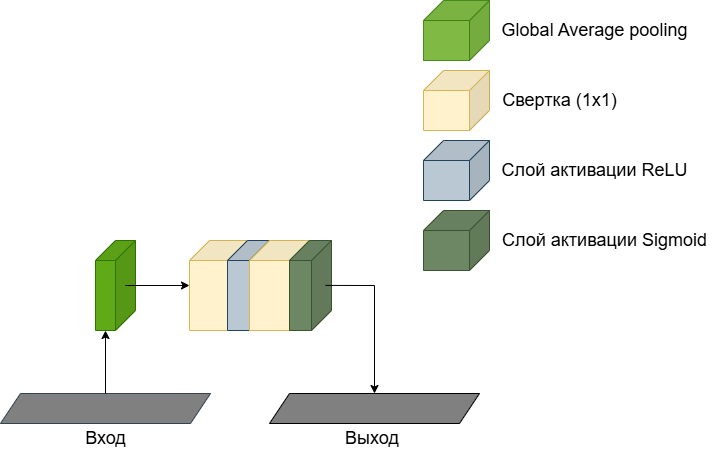
\includegraphics [scale=0.5] {my_folder/images/FocusNet-SE layer.png}
	\caption{Squeeze-and-Excitation блок}
	\label{fig:SE_block}
\end{figure}

\section{Архитектура нейросети} \label{ch2:architecture}

В основе разработанного решения лежит сверточная нейросеть MobileNet от Google, которая была разработана для классификации объектов на изображении на смартфонах. Существует несколько модификаций данной нейросети. Для решения задачи автофокуса бьла выбрана версия MobileNetV3\_Small. Одним из ключевых факторов в принятии решения была скорость работы и легковесность, так как принимать решение о смене позиции камеры нужно максимально быстро, не затрачивая больших вычислительных ресурсов.

Главная идея аданной сети -- так называемые bottleneck-блоки. Они используют depthwise свертку, преимущество которой заключается в снижении вычислительной нагрузки благодаря меньшему количеству операций и меньшем числе обучаемых параметров. В следствие этого уменьшается время обработки входных данных нейросетью, а сам алгоритм становится менее требователен к оборудованию в условиях ограниченных мощности и памяти.

Далее были внесены некоторые изменения в архитектуру MobileNet, чтобы адаптировать ее для решения поставленной задачи. Изменилась сама цель алгоритма: если оригинальная сеть предназначалась для классификации, то модифицированная версия для автофокуса должна решать задачу регрессии, так как ее цель -- предсказание непрерывной величины, а именно смещения камеры. В данном случае набором признаков (или факторов) для предсказания данной величины является само входное изображение.

Для того, чтобы адаптировать алгоритм под задачу регрессии, необходимо было внести изменения в последние слои, заменив классификатор на последовательность слоев, выполняющих регрессию. Классификатор состоял из двух полносвязных слоев, функции активации hardswish, слоя исключения (далее dropout или дропаут). Регрессор же состоит из двух полносявзных слоев и функции активации ReLU.

В качестве функции потерь была выбрана smooth L1-loss, которая является комбинацией L1-loss, также известной как Mean Absolute Error (MAE) или средняя абсолютная ошибка, и L2-loss -- Mean Squared Error (MSE) или средней-квадратичной ошибкой. Smooth L1-loss задается следующей формулой:
\begin{equation}
	L1_{smooth} =
	\begin{cases}
		\dfrac{1}{2\beta}(y-y')^2,\ |y-y'|<\beta \\
		|y-y'| - \dfrac{\beta}{2},\ \text{иначе}
	\end{cases},
\end{equation}
где $y$ -- истинное искомое значение, $y'$ -- предсказанное значение, $\beta$ -- некоторая константа, которая задается при настройке сети и в данном случае равная единице. Выбранная функция потерь имеет следующие преимущества:
\begin{enumerate}[1.]
	\item Стабильность градиента. Smooth L1-loss малых ошибок ведет себя как MSE, а для больших -- как MAE. Константа $\beta$ задает величину ошибки, на которой происходит это разделение. Но как известно, градиент функции L1-loss не определен в нуле, из-за чего могут возникать трудности при обучении во время обратного распространения ошибки. Вероятность совпадение истинного и предсказанного значений мала, но все же такое случается. Градиент функции средне-квадратичной ошибки лишен этого недостатка, но эта функция потерь вносит слишком большое влияние при больших ошибках. Градиент функции smooth L1-loss выглядит следующим образом:
	\begin{equation}
		\nabla L1_{smooth} = 
		\begin{cases}
			\dfrac{y-y'}{\beta},\ |y-y'|<\beta \\
			\text{sign}(y-y'),\ \text{иначе}
		\end{cases}
	\end{equation}
	
	Это способствует лучшей сходимости алгоритма обучения.
	
	\item Устойчивость к выбросам. Функция потерь MSE чувствительна к выбросам из-за квадратичной зависимости от ошибки. Smooth L1 при больших отклонениях ведет себя линейно, что позволяет избежать слишком большого влияния ошибок.
\end{enumerate}

Таким образом, Smooth L1-loss является некоторым симбиозом функций абсолютной и среднеквадратичной ошибки, вобрав в себя лучшее от каждой из них.

Описание архитектуры нейросети представлено в \taref{tab:nn_architecture}. Более детальную схему слоев можно увидеть на \firef{fig:FocusNet}. 

\begin{table}[!htbp]
	\centering
	\small
	\begin{tabular}{|c|c|c|c|c|c|c|}
		\hline
		Вход & Слой & exp size & Выход & SE & AF & stride\\ \hline
		$672^2 \times 3$ & conv2d, $3 \times 3$ & - & 16 & - & Hardswish & 2\\ \hline
		$336^2 \times 16$ & bneck, $3 \times 3$ & 16 & 16 & \checkmark & ReLU & 2\\ \hline
		$168^2 \times 16$ & bneck, $3 \times 3$ & 72 & 24 & - & ReLU & 2\\ \hline
		$84^2 \times 24$ & bneck, $3 \times 3$ & 88 & 24 & - & ReLU & 1\\ \hline
		$84^2 \times 24$ & bneck, $5 \times 5$ & 96 & 40 & \checkmark & Hardswish & 2\\ \hline
		$42^2 \times 40$ & bneck, $5 \times 5$ & 240 & 40 & \checkmark & Hardswish & 1\\ \hline
		$42^2 \times 40$ & bneck, $5 \times 5$ & 240 & 40 & \checkmark & Hardswish & 1\\ \hline
		$42^2 \times 40$ & bneck, $5 \times 5$ & 120 & 48 & \checkmark & Hardswish & 1\\ \hline
		$42^2 \times 48$ & bneck, $5 \times 5$ & 144 & 48 & \checkmark & Hardswish & 1\\ \hline
		$42^2 \times 48$ & bneck, $5 \times 5$ & 288 & 96 & \checkmark & Hardswish & 2\\ \hline
		$21^2 \times 96$ & bneck, $5 \times 5$ & 576 & 96 & \checkmark & Hardswish & 1\\ \hline
		$21^2 \times 96$ & bneck, $5 \times 5$ & 576 & 96 & \checkmark & Hardswish & 1\\ \hline
		$21^2 \times 96$ & conv2d, $1 \times 1$ & - & 576 & - & Hardswish & 1\\ \hline
		$21^2 \times 576$ & avgpool2d, $7 \times 7$ & - & 576 & - & - & 1\\ \hline
		$576$ & fully-connected & - & 256 & - & ReLU & -\\ \hline
		$256$ & fully-connected & - & 1 & - & - & -\\ \hline
	\end{tabular}
	\caption{Структура слоев предлагаемой нейросети}
	\label{tab:nn_architecture}	
\end{table}

\begin{figure}[ht] 
	\center
	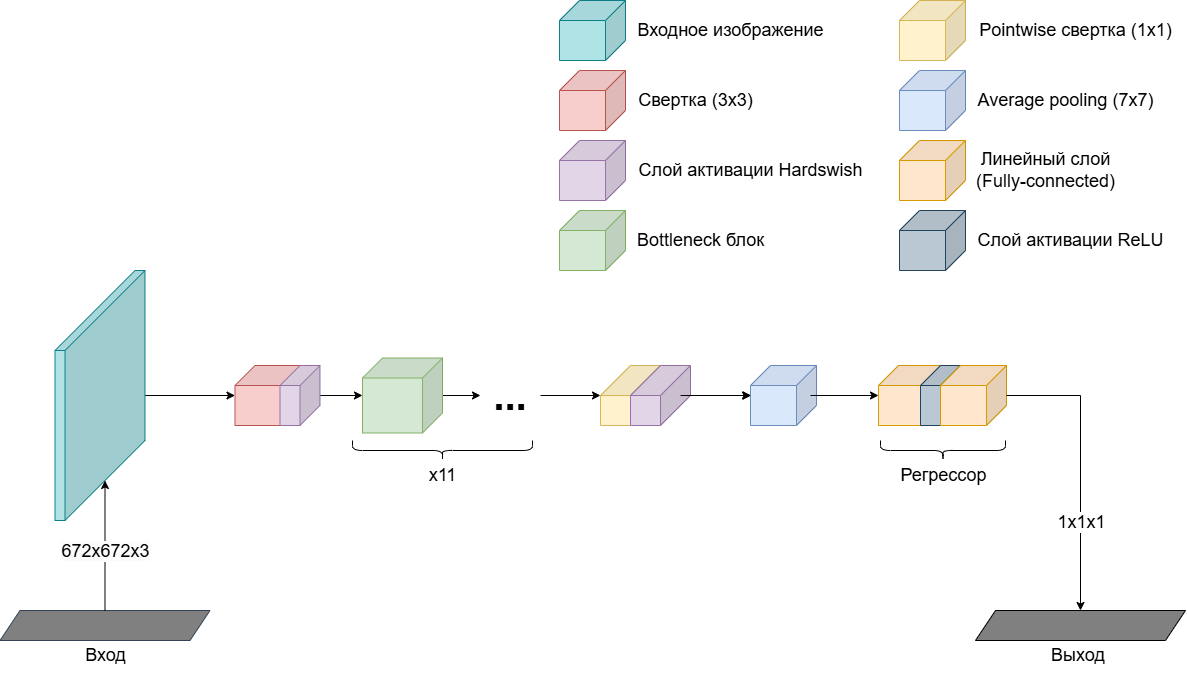
\includegraphics [scale=0.4] {my_folder/images/FocusNet-FocusNet2.png}
	\caption{Общая схема нейросети} 
	\label{fig:FocusNet}
\end{figure}

Также на \firef{fig:FocusNet-Bottleneck} представлена стуктура Bottleneck блока. Данный тип элемента можно считать ключевой инновацией, поскольку в нем используются инвертированные остаточные блоки. Особенность таких bottleneck блоков заключается в следующем:
\begin{itemize}
	\item Инвертированная структура. В традиционных остаточных блоках используется уменьшение размерности данных перед обработкой. В инвертированных блоках сначала происходит увеличение размерности, затем обработка данных, а потом сжатие обратно к исходной размерности. Это позволяет выявлять высокоуровневые признаки в условиях ограниченности вычислительных ресурсов.
	
	\item Свертка по глубине. Как уже говорилось в параграфе \ref{par:convolution}, depthwise свертка значительно уменьшает вычислительную сложность и количество обучаемых параметров.
	
	\item Squeeze-and-Excitation (SE) блоки. Эти блоки помогают адаптивно перенастраивать весовые коэффициенты каналов, усиливая важные признаки и подавляя менее значимые, что улучшает представление данных и общую производительность модели.
	
	\item Функция активации Hardswish. Эта функция проста в вычислительном смысле, помогает нейросети справляться с ленилейными зависимостями, хорошо сохраняет информацию и градиенты при отрицательных значениях входных данных.
\end{itemize}

\begin{figure}[ht] 
	\center
	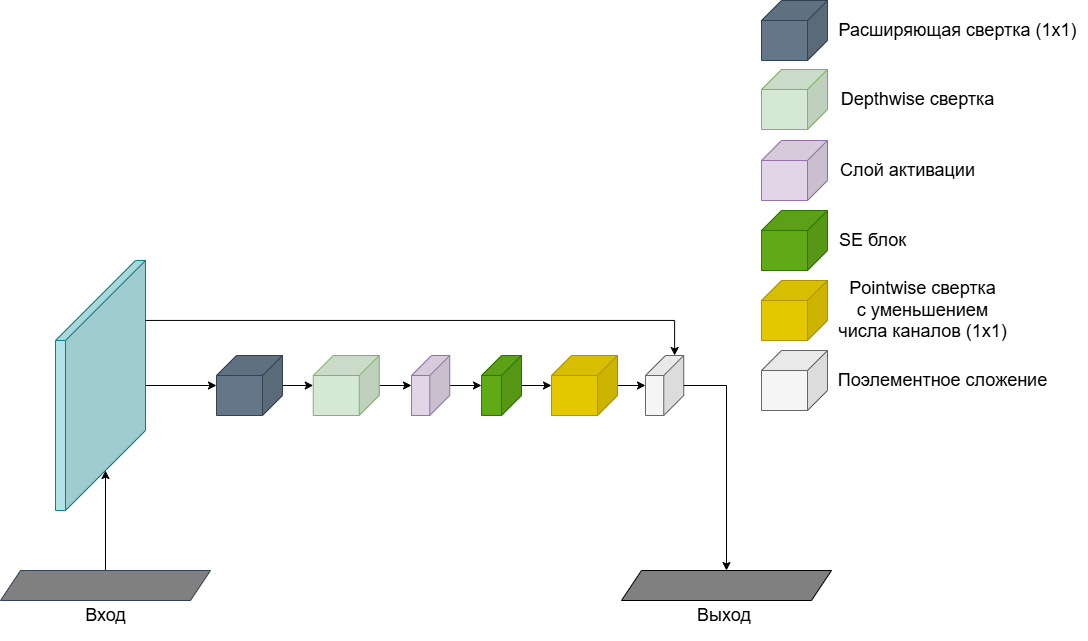
\includegraphics [scale=0.4] {my_folder/images/FocusNet-Bottleneck.png}
	\caption{Структура bottleneck блока}
	\label{fig:FocusNet-Bottleneck}
\end{figure}

\section{Определение направления смещения}
Попытка смоделировать размытое изображение (например, для обучения нейросети) с помощью простых инструментов таких, как размытие по Гауссу, приводит к тому, что между изображениями по обе стороны от фокальной плоскости, но на равном удалении нет разницы. Соответственно, в таком случае нельзя определить направление смещения камеры от объекта съемки. Однако реальная дефокусировка устроена сложнее, она содержит асимметричные хроматические и сферические аберрации. Изображение, получаемое с микроскопа в силу неидеальности систем регистрации и оптики , а также физики света является сверткой <<чистого>> изображения и функции рассеяния точки (ФРТ) \cite{sibarita2005deconvolution}. Помимо этого камера вносит свой шум в получаемое изображение. Таким образом, итоговое изображение можно описать формулой:
\begin{equation}
	I'=I \circledast H + N,
	\label{eq:res_img_with_PSF}
\end{equation}
где $I$ -- исходное изображение, $H$ -- ФРТ, $N$ -- шум от системы регистрации, $I'$ -- результирующее изображение.

Благодаря такому механизму, реальные снимки объекта по разные стороны фокальной плоскости будут отличаться. На \firef{fig:PSF} приведена оценка  асимметрии функции рассеяния точки, смоделированной на разных длинах волн и на разном расстоянии от фокальной плоскости. Хорошо видно, что противоположные друг другу изображения неодинаковые. Именно это позволяет определять направление движения камеры.

\begin{figure}[ht] 
	\center
	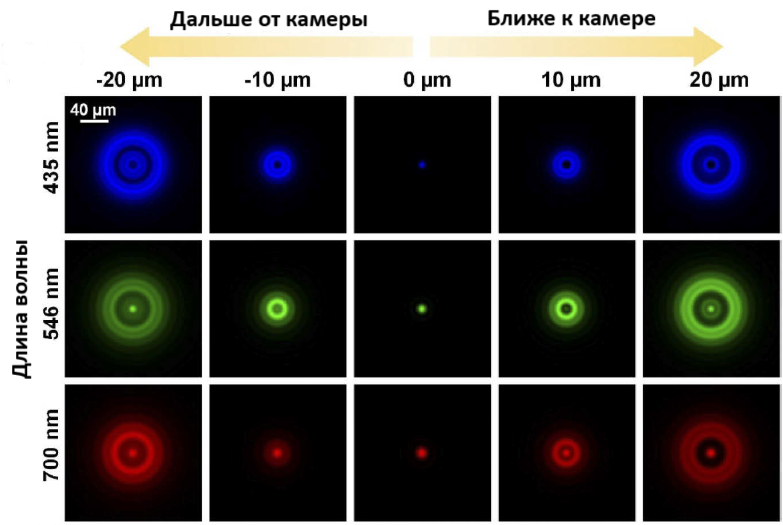
\includegraphics [scale=0.8] {my_folder/images/PSF.png}
	\caption{Смоделированные ФРТ}
	\label{fig:PSF}
\end{figure}


%% Вспомогательные команды - Additional commands
%
%\newpage % принудительное начало с новой страницы, использовать только в конце раздела
%\clearpage % осуществляется пакетом <<placeins>> в пределах секций
%\newpage\leavevmode\thispagestyle{empty}\newpage % 100 % начало новой страницы